\documentclass{article}[12pt]
\renewcommand{\baselinestretch}{1.5}
\setlength{\parskip}{1em}

\usepackage[parfill]{parskip}
\usepackage[affil-it]{authblk}
\usepackage[space]{grffile}

\usepackage[a4paper]{geometry}
\geometry{verbose}
\usepackage{float}
\usepackage{graphicx}
\graphicspath{{figures/}}
\usepackage{setspace}
\usepackage{caption}

\usepackage[utf8]{inputenc}
\usepackage[english]{babel}

\usepackage{latexsym,textcomp,longtable,tabulary}
\usepackage{booktabs,array,multirow,braket}
\usepackage{amsfonts,amsmath,amssymb,mathbbol,calc}
\usepackage{subfigure,color,blindtext,enumitem,siunitx}
\usepackage[colorinlistoftodos]{todonotes}

\usepackage{mathtools}
\usepackage{url,hyperref,etoolbox}
\numberwithin{equation}{section}
\hypersetup{colorlinks=false,pdfborder={0 0 0}}

%+figure layout options
\restylefloat{figure}
\setlist{leftmargin=*,before=\setlength{\rightmargin}{\leftmargin}}
%-figure layout options

\providecommand\citet{\cite}
\providecommand\citep{\cite}
\providecommand\citealt{\cite}

\makeatletter
\makeatother

\def\code#1{\texttt{#1}}
\begin{document}

\title{
Time-series segmentation and latent\\ representation of musical instruments
}

\author{Gregory Szep}
\affil{King's College London}
\date{\today}
\maketitle

\abstract{dd}
\section{scientific publication}
Select a scientific publication about non-equilibrium molecular dynamics of
biomolecules and discuss its relevance respect to the course you attended and
this research assignment.

\section{Unfolding proteins with umbrella sampling}
Every student has access to the raw data of umbrella sampling simulations for
two systems. These umbrella sampling simulations have been ran having the
aim to calculate the Potential of Mean Force (PMF) of the mechanical unfolding
of two peptides: one being in the initial conformational state of an a-helix; the
other being in the initial conformational state of a b-hairpin. Every student is
supposed to calculate the PMF for both the systems
\subsection{Describe the simulated systems and the type of performed simulations you
analyze}
\subsection{Calculate and display (plot) the PMF for the two systems. Explore the
relevance of the bootstrap parameter respect to evaluation of the PMF’s error
using the script g_wham_script_new.x}

Bootstrapping is a resampling method that quantifies statistical uncertainty by
dividing the data into $N$ subsets, hence without additional measruements
uncertainty is obtained by \textit{pulling the data up by its own bootstraps}.
By default the \code{g\_wham} code forms subsets with replacement over the
complete histograms along the reaction coordinate \cite{gwham2010}, leaving us
with $N$ as a hyperparameter.
\\\\
This hyperparameter is subject to the bias-variance trade-off. Chooseing a large
$N$ results in relatively unbiased and uncertain estimates, while a small number
of subsets give rise to more certain yet biased estimates. The former is
preferred but comes with a computational cost. It appears that the uncertainty
bounds converge to a fixed value after around $N\geq20$ so there is little sense
in setting $N$ at any other value than $N=20$.

\subsection{Quantify and discuss the histograms’ overlap as
obtained from the analysis of the umbrella sampling simulations}
\pagebreak
\section{Conductance of a porin}
\vspace{-5pt}
\subsection{Structure and function}
Porins are $\beta$-barrel transmembrane proteins that act as a pore through
which molecules can diffuse. Outer membrane protein F (ompF) is a nonspecific
weakly cationic selective porin found in \textit{E. Coli} \cite{Novikova2009}.
It is nonspecific in the sense that there is no preference for a particular
chemical species, however it does exhibit weak selective permeability for
cations.
\begin{figure}[H]
	\centering{}
	\captionsetup{justification=centering}
	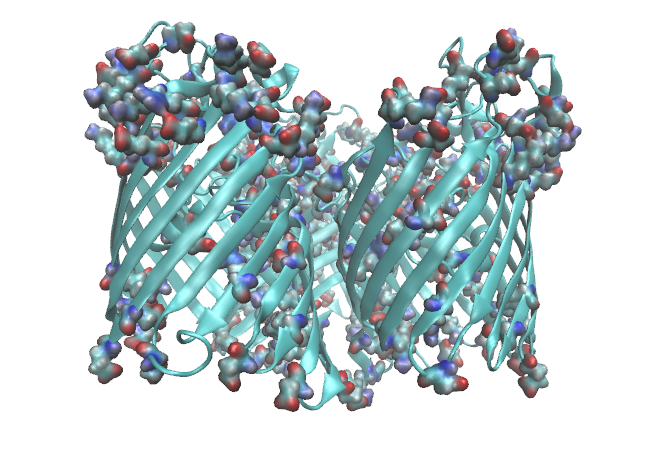
\includegraphics[scale=0.5]{ompf}
\caption{Side-view of ompF: $\beta$-barrel homotrimer forms transmembrane channel.\\
Highlighted are polar residues, which dominanate the outer membrane side.}
\label{fig:ompF}
\end{figure}\noindent
Figure \ref{fig:ompF} shows the structure of ompF: antiparallel $\beta$-strands
forming three barrels that interact locally with neighboring $\beta$-strands, a
long loop inserts into each barrel resulting in channel narrowing, charged
residues form clusters at the entrance to a pore on the outer membrane side as
well as within the narrow channel zone.
\\\\
The narrowing geometry prevents larger potentially harmful molecules such as
detergents from diffusing across the membrane, while allowing small hydrophilic
molecules involved in bacterial metabolism to pass. Charged residues in the
narrowing region of each barrel influence the ion selectivity and permeability
of the channel. Two clusters of oppositely charged residues as shown in Figure
\ref{fig:ompF-charges} generate a screw-like electric field twisted along the
channel axis with a strong transverse component in the pore narrowing region
\cite{Novikova2009}. This field favors cations to pass through the channel.
\begin{figure}[H]
	\centering{}
	\captionsetup{justification=centering}
	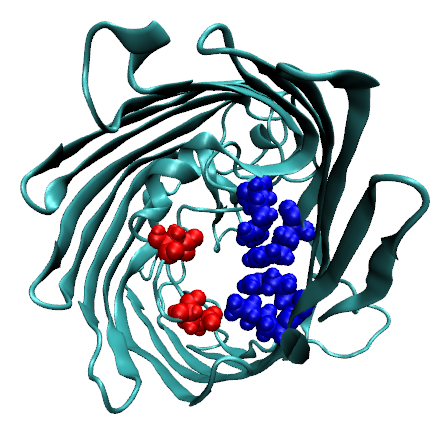
\includegraphics[scale=0.5]{ompf-charges}
\caption{ompF $\beta$-barrel from inner membrane side having residues with
positive \\ $\color{red}{\mathrm{COOH}}$ and negative $\color{blue}{\mathrm{NH_2}}$ partial
charged groups that facilitate cationic selectivity}
\label{fig:ompF-charges}
\end{figure}
\begin{figure}[H]
	\centering{}
	\captionsetup{justification=centering}
	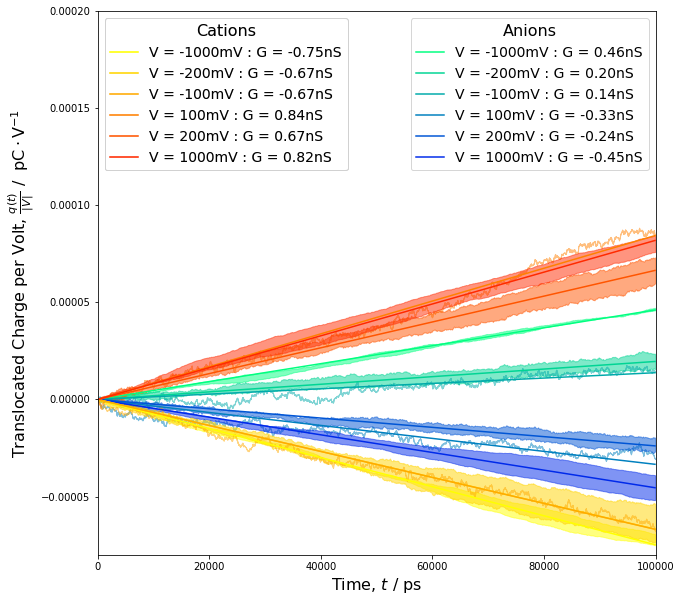
\includegraphics[scale=0.47]{conductance}
\caption{Conductance estimates $G$ from ensemble trajectories \\
for anions and cations across ompF under various applied voltages $V$ }
\label{fig:conductance}
\end{figure}

\subsection{Conductance estimates from molecular dynamics}
Classical force field molecular dynamics with an extental electric field was
used to estimate the conductance of ompF. The structure of ompF was embedded
in a lipid bilayer, surrounded by a water, Potassium $\mathrm{K^{+}}$ and
Chloride $\mathrm{Cl^{-}}$ ions. Simulations were run for up to 100ns with
external fields given by $V=\pm100\mathrm{mV},\pm200\mathrm{mV},\pm1\mathrm{V}$.
The translocated anionic and cationic charge $q(t)$ was recorded as a function of time.
Several trajectories for a given paramerer set where run to obtain a mean and
uncertainty. The cationic/anionic conductance $G_{\pm}$ was estimated via least squares according to
the formula
\begin{align}
	q(t)=G_{\pm}|V|t
\end{align}
Results summarised in Figure \ref{fig:conductance} show mean and standard
deviation for each trajectory ensemble. The claim of cationic selectivity
\cite{Benz1985} is supported as $|G_{+}|>|G_{-}|$ for all estimates and
applied voltages. Estimated conductances also share the same order of
magnitude as those reported in literature \cite{Benz1985}.

\bibliography{mendeley_v2}
\bibliographystyle{ieeetr}
\end{document}
